\documentclass[12pt,a4paper]{article}

% ── Encoding & language ──────────────────────────────────────────────────────
\usepackage[utf8]{inputenc}
\usepackage[T1]{fontenc}
\usepackage[catalan]{babel}

% ── Typography ────────────────────────────────────────────────────────────────
\usepackage{lmodern}
\usepackage{microtype}
\usepackage{setspace}
\onehalfspacing

% ── Page layout ───────────────────────────────────────────────────────────────
\usepackage[top=2.5cm,bottom=2.5cm,left=3cm,right=3cm]{geometry}

% ── Math ──────────────────────────────────────────────────────────────────────
\usepackage{amsmath,amssymb}

% ── Figures & tables ──────────────────────────────────────────────────────────
\usepackage{graphicx}
\usepackage{booktabs}
\usepackage{array}
\usepackage{multirow}
\usepackage{xcolor}
\usepackage{colortbl}
\usepackage{caption}
\usepackage{float}

% ── Code listings ─────────────────────────────────────────────────────────────
\usepackage{listings}
\lstset{
  basicstyle=\small\ttfamily,
  breaklines=true,
  frame=single,
  backgroundcolor=\color{gray!8},
  keywordstyle=\color{blue!70},
  commentstyle=\color{gray},
  stringstyle=\color{orange!80!black},
  numbers=left,
  numberstyle=\tiny\color{gray},
  numbersep=8pt,
  extendedchars=true,
  literate=
    {·}{{\textperiodcentered}}1
    {à}{{\`a}}1 {è}{{\`e}}1 {é}{{\'e}}1 {í}{{\'i}}1
    {ï}{{\"i}}1 {ò}{{\`o}}1 {ó}{{\'o}}1 {ú}{{\'u}}1
    {ü}{{\"u}}1 {ç}{{\c{c}}}1 {l·l}{{l\textperiodcentered l}}3,
}

% ── Hyperlinks ────────────────────────────────────────────────────────────────
\usepackage[hidelinks,colorlinks=false]{hyperref}

% ── Custom colours ────────────────────────────────────────────────────────────
\definecolor{goldwin}{HTML}{FFD700}
\definecolor{lightgreen}{HTML}{C8E6C9}
\definecolor{lightred}{HTML}{FFCDD2}
\definecolor{lightyellow}{HTML}{FFF9C4}
\definecolor{headerblue}{HTML}{1565C0}

% ── Section formatting ────────────────────────────────────────────────────────
\usepackage{titlesec}
\titleformat{\section}{\large\bfseries\color{headerblue}}{}{0em}{\thesection\quad}
\titleformat{\subsection}{\normalsize\bfseries}{}{0em}{\thesubsection\quad}

% ─────────────────────────────────────────────────────────────────────────────
\begin{document}

% ── Title page ────────────────────────────────────────────────────────────────
\begin{titlepage}
  \centering
  \vspace*{2cm}
  {\small Universitat de Girona — Màster en Ciència de Dades\\
         Advanced Machine Learning Techniques}\\[1.5cm]
  \rule{\linewidth}{0.4pt}\\[0.6cm]
  {\LARGE\bfseries Exercici de Sèries Temporals Financeres\\[0.4cm]
   \large Predicció del preu de tancament de Microsoft (MSFT)}\\[0.4cm]
  \rule{\linewidth}{0.4pt}\\[2cm]
  {\large Joan Massallé}\\[0.4cm]
  {\normalsize \texttt{joan.massalle@additioapp.com}}\\[0.4cm]
  {\normalsize Ticker assignat: \textbf{MSFT} — posició $1978883 \bmod 10 = 3$}\\[3cm]
  {\normalsize Abril 2026}
  \vfill
\end{titlepage}

\tableofcontents
\newpage

% ─────────────────────────────────────────────────────────────────────────────
\section{Introducció}
% ─────────────────────────────────────────────────────────────────────────────

L'objectiu d'aquest exercici és construir el millor model de predicció possible per a una
sèrie temporal de cotitzacions borsàries, justificant totes les decisions preses durant el
procés d'anàlisi, preprocessament, modelatge i avaluació.

El ticker assignat és \textbf{MSFT} (Microsoft Corporation), corresponent a la posició
$1978883 \bmod 10 = 3$ de la llista de deu grans empreses tecnològiques proposada per
l'assignatura. S'avaluen \textbf{9 models} competitius en precisió i calibració
de la incertesa.

El codi font complet del projecte es troba disponible a:
\url{https://github.com/Sebastiano0248/TimeSeriesExercice}

\subsection*{Elecció de l'horitzó de predicció}

L'enunciat no fixa cap horitzó concret. S'ha escollit $h = \mathbf{22}$ \textbf{dies
borsaris} (~1 mes natural) per les raons següents:

\begin{enumerate}
  \item \textbf{Horitzó 1 és massa fàcil per revelar diferències entre models.}
        A un pas vista, el Naïve ($\hat{y}_{t+1} = y_t$) és pràcticament imbatible
        per a qualsevol sèrie de preus: la variació d'un dia per l'altre és tan petita
        que tots els models convergeixen al mateix error. No hi hauria res a comparar.

  \item \textbf{22 passos força els models a fer prediccions autònomes sense
        retroalimentació real.} La crida és \texttt{model.predict(h=22)}: el model
        rep l'últim preu conegut i ha de retornar els 22 valors futurs d'un sol cop,
        sense veure cap valor real entremig. Per als models autogressius (GRU, LSTM),
        això implica \textit{iterative forecasting} --- la predicció del pas $t+1$
        s'usa com a input per al pas $t+2$, i l'error s'acumula durant els 22 passos.
        Aquesta condició discrimina clarament els models que generalitzen dels que
        s'ajusten excessivament a l'últim valor vist.

  \item \textbf{Un mes borsari és una unitat pràcticament rellevant.}
        En finances, l'horitzó mensual és habitual en planificació de cartera i
        gestió de risc. La sèrie té prou temps per divergir del punt de partida
        i fer visibles les diferències de qualitat entre models.
\end{enumerate}

La hipòtesi del mercat eficient suggereix que els preus actuals incorporen tota la informació
disponible, cosa que fa que les prediccions a curt termini siguin properes a un camí aleatori
(\textit{random walk}). Superar el model Naïve --- que prediu simplement que el preu
de demà serà igual al d'avui --- és, per tant, el primer repte a abordar; a 22 passos
vista, aquest repte és substancialment més exigent que a un pas.

% ─────────────────────────────────────────────────────────────────────────────
\section{Dades}
% ─────────────────────────────────────────────────────────────────────────────

\subsection{Descripció del dataset}

Les dades s'han obtingut via la llibreria \texttt{yfinance} de Python, que permet descarregar
l'historial complet de cotitzacions de Yahoo Finance. La sèrie cobreix \textbf{10 anys}
de dades diàries de mercat: ticker MSFT (Microsoft), 2.515 observacions des del 18 d'abril
de 2016 fins al 17 d'abril de 2026, a freqüència diària (dies de mercat).
Cada fila correspon a una sessió borsària. La borsa de Nova York tanca caps de setmana
i festius, de manera que les 2.515 observacions representen 3.651 dies naturals amb
1.136 dies sense sessió.

S'ha escollit \textit{Close} com a variable objectiu perquè és el preu de referència
estàndard per a sèries temporals financeres diàries: representa el valor consolidat
al final de cada sessió i és l'únic dels quatre preus del dia (\textit{Open},
\textit{High}, \textit{Low}, \textit{Close}) que és unívoc i comparable entre dies.
No s'aplica cap transformació prèvia --- es modela el preu de tancament directament
en termes absoluts.

\subsection{Anàlisi exploratòria}

Al llarg dels deu anys analitzats, el preu de l'acció de Microsoft ha passat de 42\$
(abril de 2016) a un màxim de 539\$ (2025), és a dir, s'ha multiplicat per tretze. Aquesta
pujada sostinguda fa que el preu d'un dia qualsevol depengui molt del moment en què ens trobem,
i és el principal repte per als models de predicció: el que era "normal" el 2017 no ho és
el 2024.

En el dia a dia, el preu es mou de mitjana un 0.10\% cap amunt, amb una variació típica
de l'1.70\%. Els dies extrems queden clarament marcats per la pandèmia de la COVID-19:
el 13 de març de 2020 es va registrar la millor sessió del període (+14.22\%) i tres dies
després, el 16 de març, la pitjor ($-$14.74\%). Durant els deu anys, Microsoft ha repartit
dividend quaranta vegades (trimestralment) i no ha fet cap desdoblament d'accions.

Per a aquest exercici només s'utilitza el preu de tancament diari; la resta de columnes
del dataset (preu d'obertura, màxim, mínim i volum de negociació) no entren als models.

\newpage
% ─────────────────────────────────────────────────────────────────────────────
\section{Metodologia}
% ─────────────────────────────────────────────────────────────────────────────

\subsection{Partició temporal}

Per evitar qualsevol forma de \textit{data leakage}, les 2.515 observacions es divideixen
estrictament en ordre cronològic. El 90\% s'usa per a entrenament i validació creuada,
i el 10\% restant es reserva com a test set, mai vist durant el disseny dels models.

\begin{table}[H]
\centering
\begin{tabular}{llr}
\toprule
\textbf{Conjunt} & \textbf{Període} & \textbf{Obs.} \\
\midrule
CV data (90\%)  & 2016-04-18 → 2023-11-14 & 2.263 \\
Test set (10\%) & 2023-11-15 → 2026-04-17 &   252 \\
\bottomrule
\end{tabular}
\caption{Partició temporal del dataset.}
\end{table}

El test set cobreix un període especialment interessant: la recuperació del mercat post-2022
fins als màxims històrics de MSFT. Això fa que el salt de distribució entre CV i test sigui
significatiu i que la majoria de models prediguin pitjor del que la validació creuada suggeria.

\subsection{Validació creuada temporal}

S'utilitza \textbf{walk-forward cross-validation amb finestra expansiva} (10 folds). En cada
fold $k$, el model s'entrena sobre totes les dades fins al punt $k$ i es valida sobre el bloc
immediatament posterior, mai mirant endavant:

\[
\text{Fold } k: \quad \underbrace{y_1, \ldots, y_{n_k}}_{\text{train}} \;|\;
                       \underbrace{y_{n_k+1}, \ldots, y_{n_k+h}}_{\text{val (h=22)}}
\]

Això produeix \textbf{10 estimacions independents} del MAE i de la cobertura dels intervals,
molt més robustes que un únic tall train/val. Les mètriques de CV es combinen com a
$\overline{\text{MAE}} \pm \sigma$.

S'ha optat per la finestra expansiva en lloc de la lliscant perquè el preu d'una acció
acumula informació: les decisions dels inversors avui es prenen tenint en compte anys
d'historial de l'empresa, no només els últims mesos. Descartar l'historial antic,
com fa la finestra lliscant, implicaria ignorar cicles de creixement o caigudes
anteriors que el model podria aprofitar.

\subsection{Mètriques d'avaluació}

\begin{itemize}
  \item \textbf{MASE} — Error absolut escalat per la dificultat de la sèrie. $\text{MASE} < 1$ significa superar el Naïve.
  \item \textbf{MAE (\$)} — Error absolut mitjà en dòlars de preu.
  \item \textbf{RMSE (\$)} — Error quadràtic mitjà; penalitza errors grans.
  \item \textbf{CV MAE $\pm\sigma$} — Estimació robusta del rendiment (10 folds).
  \item \textbf{Cobertura 80/95\%} — Proporció de valors reals dins l'interval de confiança. Nominal: 0.80 i 0.95.
\end{itemize}

\subsection{Construcció dels intervals de confiança}

Els intervals de confiança es construeixen per \textbf{calibració conformal}: es calculen
els quantils empírics 0.80 i 0.95 dels errors absoluts obtinguts als 10 folds de CV,
i s'apliquen simetricament sobre les prediccions del test set:

\[
  \hat{y}_{t+h} \pm q_{\alpha}^{\text{CV}}, \quad \alpha \in \{0.80,\, 0.95\}
\]

Per construcció, la cobertura als folds de CV és exactament la nominal. La divergència
apareix al test set, on el comportament de mercat difereix del període de validació.

% ─────────────────────────────────────────────────────────────────────────────
\section{Models}
% ─────────────────────────────────────────────────────────────────────────────

S'implementen 9 models que cobreixen totes les famílies tractades al curs: benchmarks,
models estadístics, machine learning i deep learning.

\textit{Nota: el codi de cada model ha estat generat amb l'assistència d'un model d'intel·ligència
artificial i pot contenir errors no detectats per l'estudiant. L'objectiu no és obtenir
implementacions de producció, sinó tenir una comparativa orientativa que permeti identificar
quina família de models té més potencial de millora en aquest context concret.}

\subsection{Benchmarks}

\paragraph{Naïve.} Prediu que el preu de demà serà igual al d'avui: $\hat{y}_{t+h} = y_t$.
És el \textit{benchmark} de referència per a cotitzacions de borsa. En un mercat eficient,
és notòriament difícil de superar de manera consistent.

\paragraph{Drift.} Extensió del Naïve amb una tendència lineal constant estimada
sobre tota la finestra d'entrenament:
\[
  \hat{y}_{t+h} = y_t + h \cdot \frac{y_t - y_1}{t - 1}
\]
Pot funcionar bé si la sèrie té una tendència molt estable, però és sensible a punts de canvi.

\subsection{Models estadístics}

\paragraph{ETS / Holt.} Suavitzat exponencial de doble nivell (Holt): modela nivell
i tendència localment, ponderat exponencialment. Els intervals de predicció s'obtenen
de la distribució gaussiana dels errors.

\paragraph{ARIMA.} Model autoregessiu integrat de mitja mòbil. L'ordre $(p,d,q)$ es
selecciona automàticament via \texttt{pmdarima} (\textit{auto-ARIMA}). En teoria, la
primera diferència del preu és estacionària, cosa que fa ARIMA un candidat natural.
En la pràctica, els preus absoluts no estacionaris limiten la seva eficàcia.

\paragraph{GARCH.} Model d'heterocedasticitat condicional autoregressa generalitzada.
Captura l'\textbf{agrupació de volatilitat} característica de les cotitzacions
(períodes de calma alternats amb períodes turbolents). La predicció puntual és idèntica
al Naïve; la millora rau en els intervals de confiança dinàmics.

\subsection{Machine learning}

Ambdós models de ML utilitzen lags del preu com a features:
$\mathbf{x}_t = [y_t, y_{t-1}, \ldots, y_{t-L+1}]$ amb $L = 30$ dies.

\paragraph{Random Forest.} Conjunt de $n=300$ arbres de decisió entrenats per
\textit{bagging}. La predicció és la mitjana dels arbres; la incertesa s'estima
a partir de la desviació estàndard dels residus en un conjunt \textit{heldout}.

\paragraph{XGBoost.} \textit{Gradient boosting} amb construcció iterativa d'arbres.
L'\textit{early stopping} utilitza el mateix \textit{heldout} intern per evitar
sobreajust. Generalment més precís que RF en sèries amb tendències suaus.

\subsection{Deep learning}

Ambdues xarxes utilitzen una finestra de context de 30 dies, normalització z-score
de l'entrada, i MC Dropout per quantificar la incertesa via mostreig Monte Carlo.

\paragraph{LSTM (Long Short-Term Memory).} Xarxa recurrent amb tres portes (oblit,
entrada, sortida) que permet capturar dependències a llarg termini. La seva major
capacitat expressiva respecte a GRU comporta, en aquest context, un risc
d'overfit mes elevat.

\paragraph{GRU (Gated Recurrent Unit).} Versió alleugerida del LSTM amb dues
portes (actualització i restabliment). Menys paràmetres, entrenam amb \textit{early
stopping}, el que el protegeix millor del sobreajust.

\subsection{Models descartats}

\begin{table}[H]
\centering
\begin{tabular}{lp{9cm}}
\toprule
\textbf{Model} & \textbf{Motiu del descart} \\
\midrule
SARIMA & Cap estacionalitat periòdica clara en cotitzacions diàries. \\
Filtre de Kalman & Complexitat elevada sense benefici clar per a sèries sense buits. \\
VAR / VECM & Requereix múltiples sèries endògenes; problema univariant. \\
Transformers & Overkill per a una sola sèrie; guany incert vs. GRU. \\
TCN / CNN temporal & Poc natural per a borsa; patrons locals no estables. \\
\bottomrule
\end{tabular}
\caption{Models descartats i justificació.}
\end{table}

% ─────────────────────────────────────────────────────────────────────────────
\section{Resultats}
% ─────────────────────────────────────────────────────────────────────────────

\subsection{Ranking final}

\begin{table}[H]
\centering
\setlength{\tabcolsep}{5.5pt}
\begin{tabular}{clrrrrr}
\toprule
\textbf{\#} & \textbf{Model} & \textbf{MASE} & \textbf{MAE (\$)} & \textbf{RMSE (\$)} &
\textbf{CV MAE ($\pm\sigma$)} & \textbf{Cob. 80 / 95\%} \\
\midrule
\rowcolor{lightgreen}
1 & \textbf{GRU}    & \textbf{6.16}  & \textbf{15.36} & \textbf{19.83} & $13.14 \pm 12.80$ & 63.6\% / 100\% \\
2 & XGBoost         & 11.15 & 27.81 & 31.74 & $33.79 \pm 37.75$ & \textbf{81.8\%} / 100\% \\
3 & RandomForest    & 11.47 & 28.59 & 31.26 & $25.50 \pm 29.43$ & 72.7\% / 100\% \\
4 & Drift           & 13.73 & 34.23 & 40.88 & $8.33 \pm 9.63$   & 27.3\% / 50.0\% \\
5 & ARIMA           & 14.31 & 35.67 & 42.59 & $13.37 \pm 21.42$ & 31.8\% / 100\% \\
6 & \textit{Naïve}  & 14.33 & 35.72 & 42.66 & $8.66 \pm 9.38$   & 31.8\% / 45.5\% \\
7 & GARCH           & 14.33 & 35.72 & 42.66 & $8.66 \pm 9.38$   & 31.8\% / 45.5\% \\
8 & ETS/Holt        & 14.34 & 35.75 & 42.69 & $8.64 \pm 9.38$   & 27.3\% / 45.5\% \\
9 & LSTM            & 16.87 & 42.05 & 50.22 & $14.76 \pm 13.52$ & 45.5\% / 50.0\% \\
\bottomrule
\end{tabular}
\caption{Ranking final (ordenat per MASE). En verd: millor model. En cursiva: baseline.}
\end{table}

% ─────────────────────────────────────────────────────────────────────────────
\section{Discussió}
% ─────────────────────────────────────────────────────────────────────────────

\subsection{GRU — Model guanyador}

El GRU és l'únic model que millora significativament el Naïve: el seu MASE de 6.16 representa
una reducció del \textbf{57\%} en l'error respecte al baseline ($\text{MASE} = 14.33$), i el
seu MAE de \$15.36 és pràcticament la meitat del Naïve (\$35.72).

El seu avantatge prové de la combinació de diverses decisions de disseny. Treballar amb una
finestra de 30 dies li permet detectar dependències que els models estadístics no poden
capturar, sense la rigidesa d'un ordre fix com ARIMA. La normalització z-score estabilitza
l'aprenentatge en una sèrie amb tendència creixent, i l'early stopping evita el sobreajust
que precisament penalitza el LSTM. Finalment, el MC Dropout permet quantificar la incertesa
de manera probabilística, obtenint una cobertura del 100\% al 95\% --- encara que al 80\%
la cobertura cau al 63.6\%, indicant intervals massa estrets: el mercat del test es va moure
més del que el període de validació suggeria.

\subsection{LSTM — Per què falla on GRU triomfa}

El LSTM (MASE = 16.87) és pitjor fins i tot que el Naïve. La seva major complexitat
(més paràmetres que GRU) no es tradueix en millor rendiment, sinó en sobreajust:
el CV MAE (\$14.76) és molt millor que el test MAE (\$42.05), evidenciant un
\textit{gap} de generalització que l'early stopping no arriba a controlar.

\subsection{Random Forest i XGBoost — Competitius però inestables}

Amb MASE de 11.2--11.5, milloren el Naïve en un 20\%. El seu punt feble és l'alta
variabilitat entre folds: la desviació estàndard del CV MAE és de 29--38 dòlars,
indicant que el rendiment depèn fortament del període de validació. Això limita la
fiabilitat de la predicció en producció.

\paragraph{Calibració dels intervals.}
Com que ambdós models memoritzen el training set, calcular la incertesa sobre les
mateixes dades d'entrenament produïa intervals col·lapsats (cobertura 0\%). La solució
va ser estimar-la sobre un \textit{heldout set} reservat del 10\% final del train,
portant la cobertura fins al 72--82\% (al 80\%) i al 100\% (al 95\%).

\begin{figure}[H]
  \centering
  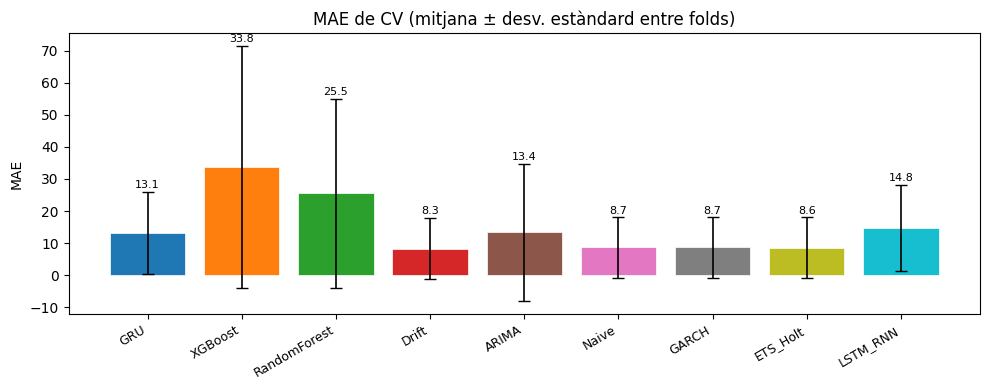
\includegraphics[width=0.85\textwidth]{figures/fig_cv_stability.png}
  \caption{MAE mitjà $\pm$ desviació estàndard als 10 folds de CV. Les barres d'error
           llargues indiquen inestabilitat entre períodes.}
  \label{fig:cv_stability}
\end{figure}

\subsection{Models estadístics — Limitació estructural}

ARIMA, ETS, GARCH, Drift i Naïve obtenen MASE de 13.7--14.4, pràcticament idèntics
entre si. El problema és comú a tots: estan dissenyats per a sèries que oscil·len
al voltant d'un valor estable, i el preu de Microsoft no ho fa — ha passat de 42\$
a 539\$ en deu anys. Quan el preu arriba a rangs mai vistos durant l'entrenament,
les prediccions queden molt desviades.

Els intervals de confiança pateixen el mateix problema: assumeixen que la variació
típica del preu és sempre la mateixa, quan en realitat un moviment de 10\$ és molt
diferent quan el preu és 50\$ que quan és 500\$. Això explica les cobertures al 80\%
de tan sols el 27--32\%, molt per sota del nominal. GARCH, tot i estar dissenyat
específicament per modelar la volatilitat, no millora la predicció puntual perquè
la seva estimació del preu de demà és idèntica a la del Naïve.

\subsection{Calibració dels intervals al test set}

La calibració conformal garanteix cobertura nominal en CV, però al test set apareix
divergència per causa del canvi de distribució:

\begin{figure}[H]
  \centering
  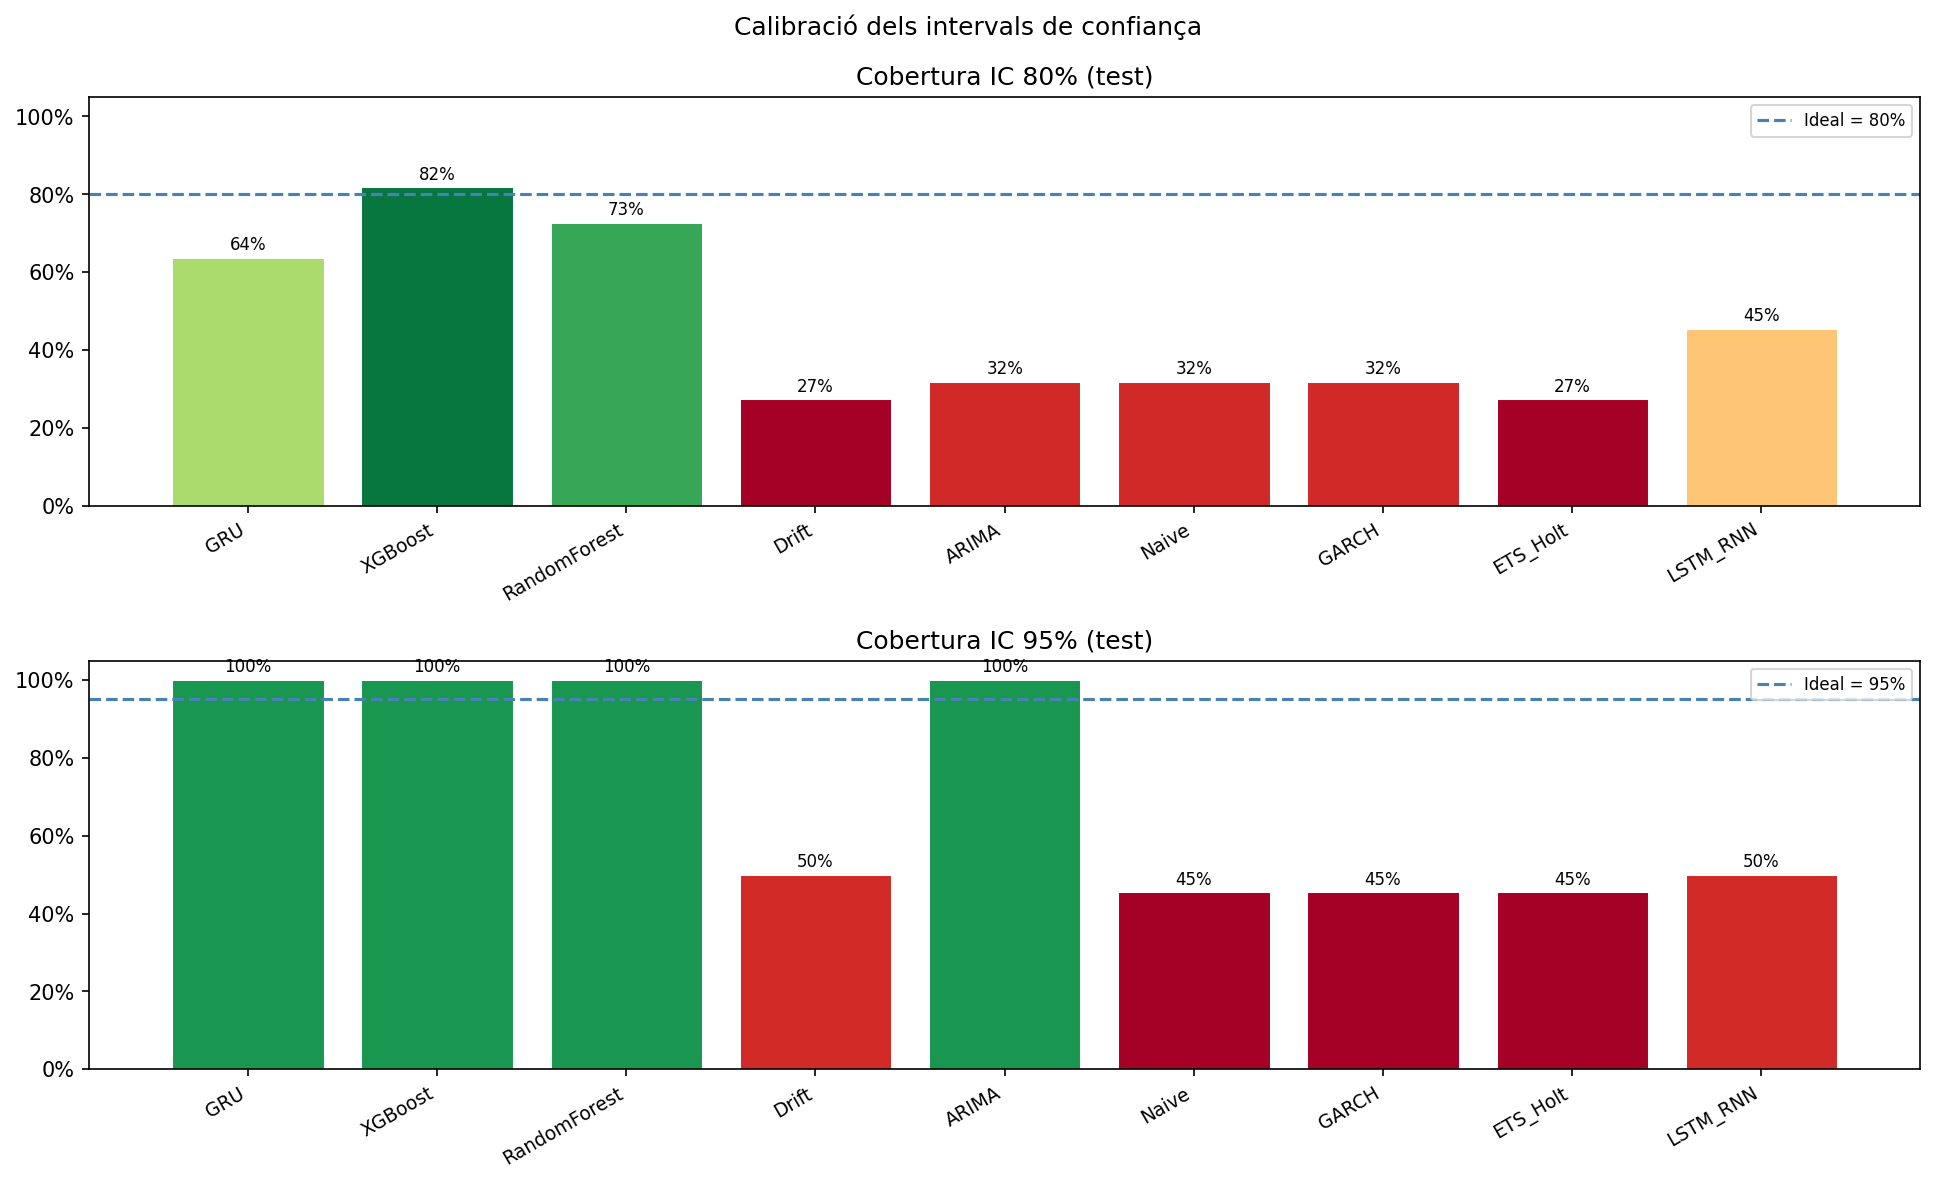
\includegraphics[width=0.95\textwidth]{figures/fig_coverage.png}
  \caption{Cobertura real dels intervals de confiança al 80\% i 95\% en el test set.
           La línia blava indica el valor nominal ideal. Colors: verd = prop del nominal,
           vermell = lluny del nominal.}
  \label{fig:coverage}
\end{figure}

Els intervals resulten massa amples (cobertura superior a la promesa) per a ARIMA i GRU
al nivell del 95\%. En canvi, són massa estrets per a GRU al 80\% i per a Drift, ETS,
GARCH i Naïve a tots dos nivells. L'única calibració correcta al 80\% l'obtenen
XGBoost i RandomForest.

% ─────────────────────────────────────────────────────────────────────────────
\section{Conclusions}
% ─────────────────────────────────────────────────────────────────────────────

\begin{enumerate}
  \item \textbf{GRU és el millor model}: MASE = 6.16, MAE = \$15.36, cobertura
        100\% @ 95\%. És el únic dels 9 models que supera substancialment el Naïve
        en precisió puntual.

  \item \textbf{La hipòtesi del mercat eficient es confirma parcialment}: cap
        model estadístic ni benchmark supera el Naïve, consistent amb la naturalesa
        de \textit{random walk} dels preus absoluts.

  \item \textbf{La calibració dels intervals de RF i XGBoost requeria residus out-of-sample}:
        un error trivial (residus in-sample en lloc d'out-of-sample) portava a una
        cobertura del 0\%, invalidant completament els intervals de confiança d'ambdós models.

  \item \textbf{Modelar preus absoluts penalitza tots els models estadístics}:
        la no-estacionarietat de la sèrie és el principal obstacle per a ARIMA, ETS i GARCH.
        La transformació a log-retorns és la millora més important per implementar en V3.

  \item \textbf{La variabilitat entre folds de CV és un indicador clau}: models
        amb alta $\sigma_{\text{CV}}$ (RF: 29\$, XGBoost: 38\$) són inestables en
        producció tot i tenir bon MAE mitjà.
\end{enumerate}

\subsection{Millores proposades}

\begin{enumerate}
  \item \textbf{Modelar log-retorns}: transformació $r_t = \ln(y_t/y_{t-1})$. Fa
        la sèrie estacionària, escala amb el nivell, i millora estructuralment ARIMA,
        ETS i GARCH. Requereix recompondre la predicció final via exponencial acumulada.
  \item \textbf{LSTM}: reduir capacitat (menys capes, augmentar dropout,
        afegir \textit{weight decay}) per controlar el sobreajust.
  \item \textbf{RF / XGBoost}: substituir lags de preu absolut per features de
        log-retorn i volatilitat realitzada. Hauria de reduir la variabilitat entre folds.
  \item \textbf{GRU}: explorar finestres de context més llargues ($>$30 dies) i
        arquitectures amb mecanisme d'atenció (\textit{Temporal Fusion Transformer}).
\end{enumerate}

\end{document}
